\usepackage{tikz}
\usetikzlibrary{positioning, shapes.multipart, fit, arrows.meta}

\begin{figure}[ht]
\centering
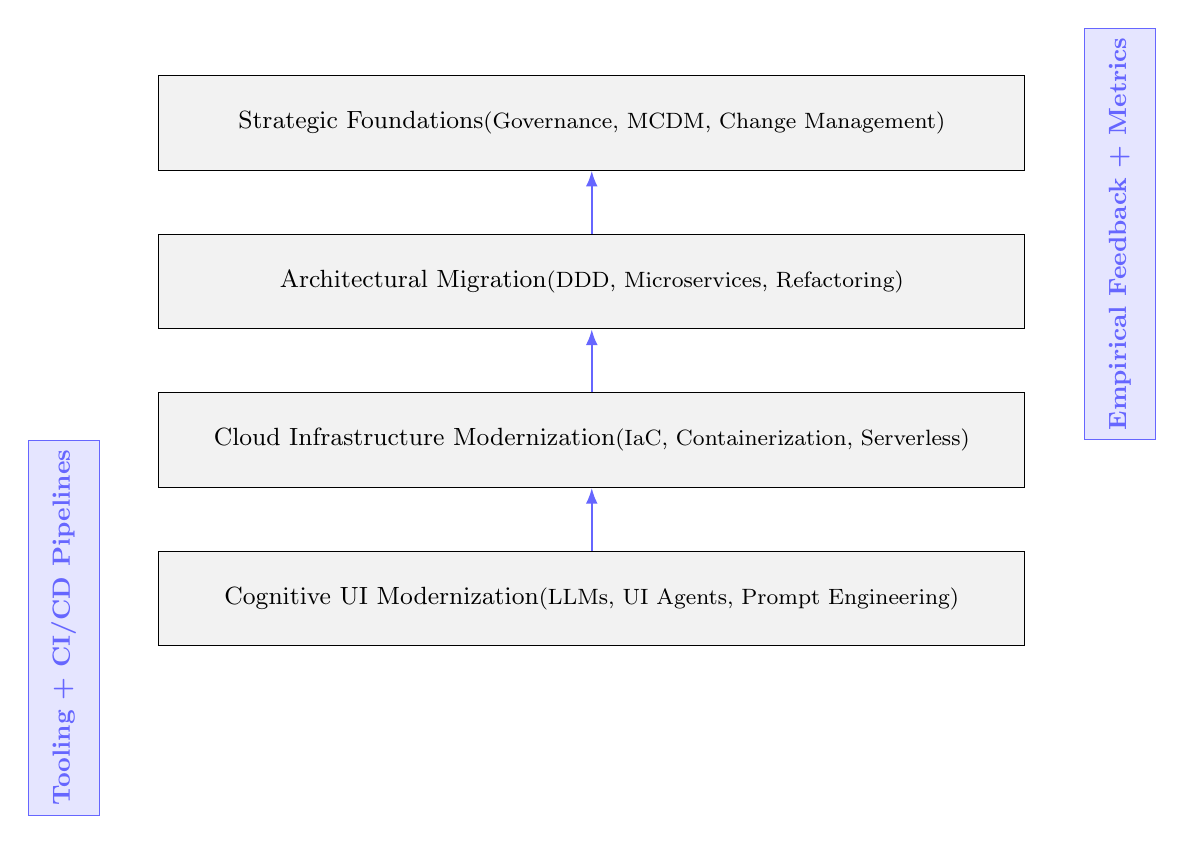
\begin{tikzpicture}[
    node distance=0.8cm,
    every node/.style={font=\small},
    layer/.style={rectangle, draw=black, fill=gray!10, minimum width=11cm, minimum height=1.2cm, text centered},
    vertical/.style={rectangle, draw=blue!60, fill=blue!10, rotate=90, anchor=center, minimum width=4.5cm, minimum height=0.9cm, text=blue!60, font=\bfseries\small},
    arrow/.style={-{Latex[length=2mm]}, thick, blue!60},
]

% Horizontal Layers
\node[layer] (layer1) at (0,3.6) {Strategic Foundations \\ \footnotesize (Governance, MCDM, Change Management)};
\node[layer, below=of layer1] (layer2) {Architectural Migration \\ \footnotesize (DDD, Microservices, Refactoring)};
\node[layer, below=of layer2] (layer3) {Cloud Infrastructure Modernization \\ \footnotesize (IaC, Containerization, Serverless)};
\node[layer, below=of layer3] (layer4) {Cognitive UI Modernization \\ \footnotesize (LLMs, UI Agents, Prompt Engineering)};

% Arrows
\draw[arrow] (layer4.north) -- (layer3.south);
\draw[arrow] (layer3.north) -- (layer2.south);
\draw[arrow] (layer2.north) -- (layer1.south);

% Cross-cutting vertical layers
\node[vertical, left=1.2cm of layer3.west] (vleft) {Tooling + CI/CD Pipelines};
\node[vertical, right=1.2cm of layer3.east] (vright) {Empirical Feedback + Metrics};

\end{tikzpicture}
\caption{Modernization Reference Framework: Functional Layers with Cross-Cutting Concerns}
\label{fig:modernization-framework}
\end{figure}
